\chapter{Survey Results}
\label{survey-results}

\section{Basic Information}
\begin{enumerate}
\begin{figure}[h]
\centering
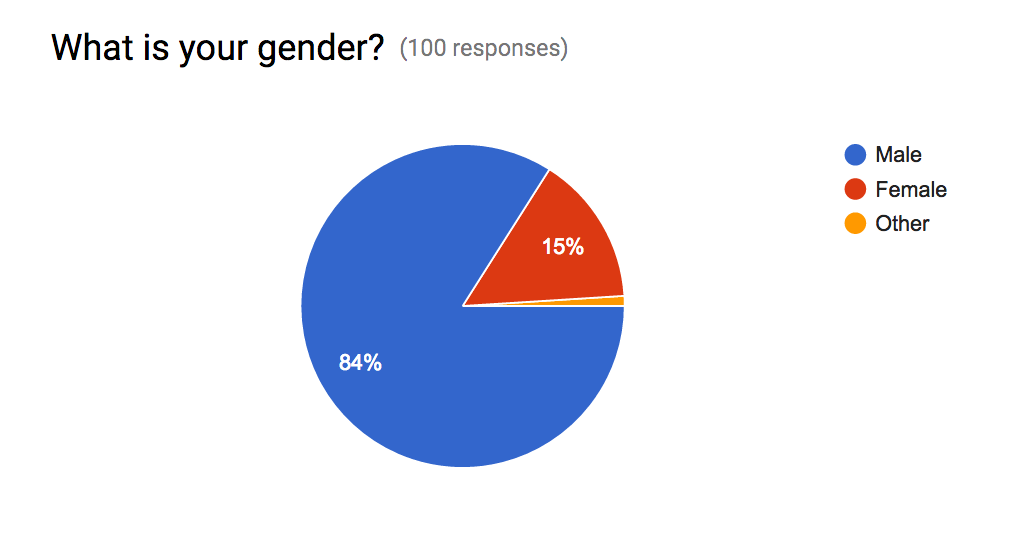
\includegraphics[width=1.0\textwidth]{sr-gender}
\caption{Gender distribution.}
\end{figure}
\item \textit{What is your gender?}
In Fall 2016, there was a total of 445 ICS students. Of the 445, 366 identified as male and 79 identified as female. This means that there was roughly 18\% females and 82\% males. The distribution of my survey has close proportions: 15\% female, 84\% male, and 1\% other. 
\begin{figure}[h]
\centering
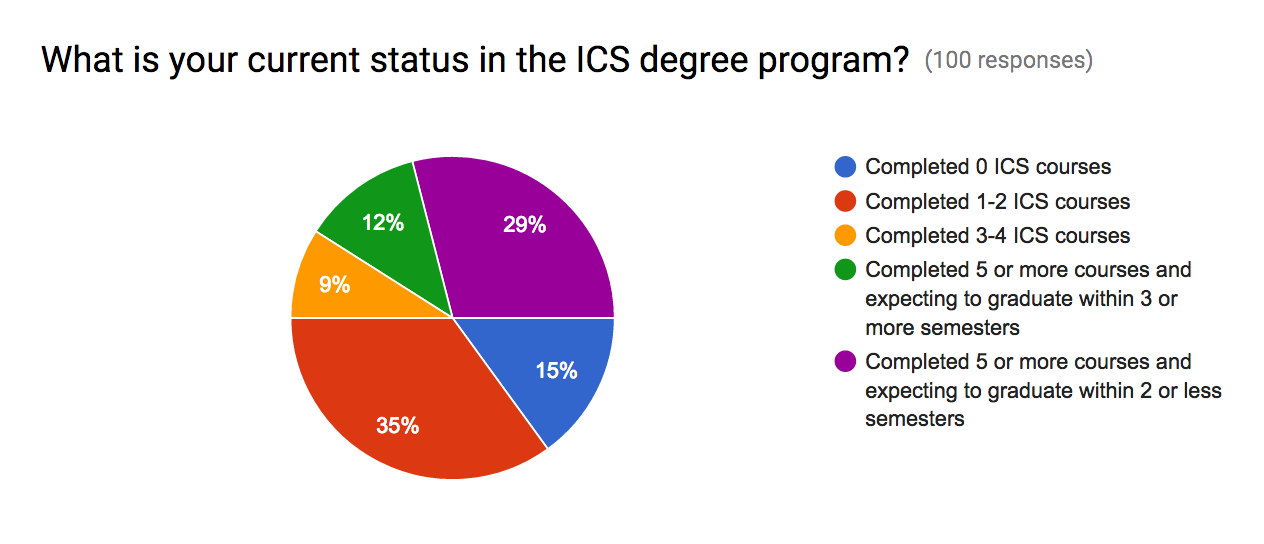
\includegraphics[width=1.0\textwidth]{sr-program-status}
\caption{ICS program status distribution.}
\end{figure}
\item \textit{What is your current status in the ICS degree program?}
The two most represented groups in the survey are those that had completed 1-2 ICS courses (35\%) and those that had completed 5 or more courses and expected to graduate within 3 or more semesters (29\%). 15\% of students surveyed were either in or about to start their first semester of ICS. Together, students who were in the middle of the program (completed 3-4 courses or 5 or more courses and expected to graduate within 3 or more semesters) comprised of 21\% of the total population surveyed. The fact that most of the students surveyed were either in the beginning of the program or about to graduate can be attributed to the fact that these are the students that physically go in for advising the most. 
\end{enumerate}

\section{Prospective ICS Students}
\begin{enumerate}
\begin{figure}[h]
\centering
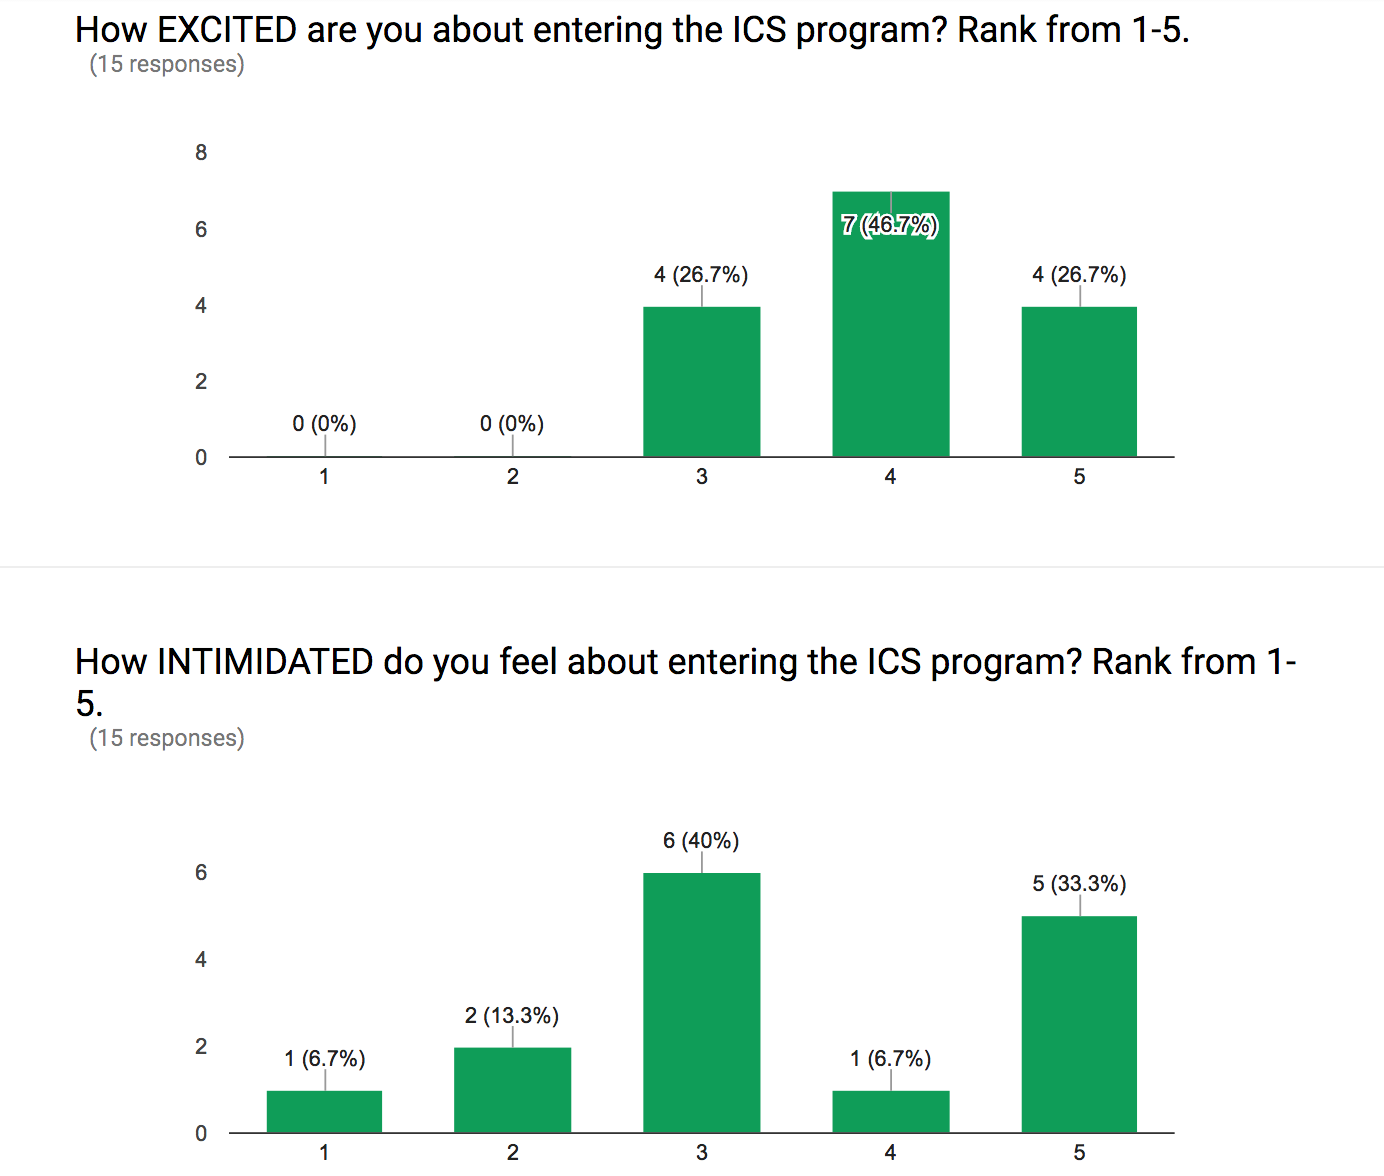
\includegraphics[width=1.0\textwidth]{sr-excited-intimidated}
\caption{Results for prospective ICS Students survey}
\end{figure}
\item\textit{How EXCITED are you about entering the ICS program? Rank from 1-5.}
The results of the survey show that all of the students surveyed felt either neutral or excited about entering the ICS program. No students stated that they were not excited. Further studies would be required to understand more behind the outside factors that affect incoming students' perceptions of the department. 
\item \textit{How INTIMIDATED do you feel about entering the ICS program? Rank from 1-5.}
The results of the survey show that a majority of the students surveyed (12 out of 15) felt either neutral or intimidated about entering the ICS program. None of the females surveyed felt less than neutral in regards to intimidation, while three males did feel less than neutral. Further studies would be required to understand more behind the outside factors that affect incoming students' feelings towards the department, and to understand if there are any differences in feelings between genders.
\end{enumerate}

\section{Current ICS Students}
\begin{enumerate}
\begin{figure}[h]
\centering
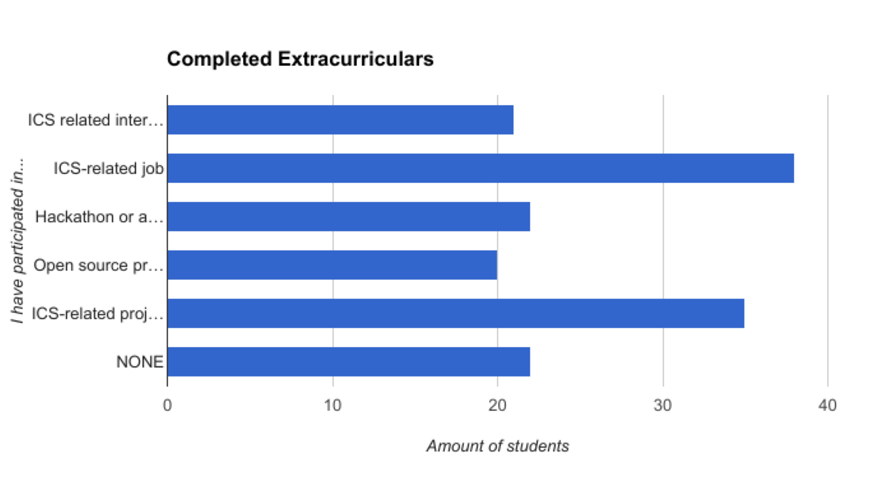
\includegraphics[width=1.0\textwidth]{sr-extracurric-bar}
\caption{Results for extracurricular participation by event type.}
\end{figure}

\begin{figure}[h]
\centering
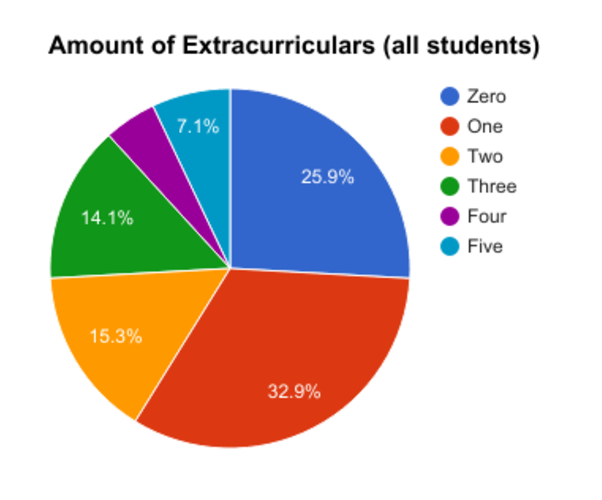
\includegraphics[width=1.0\textwidth]{sr-extracurric-pie}
\caption{Results for extracurricular participation by amount of participation (all students).}
\end{figure}

\begin{figure}[h]
\centering
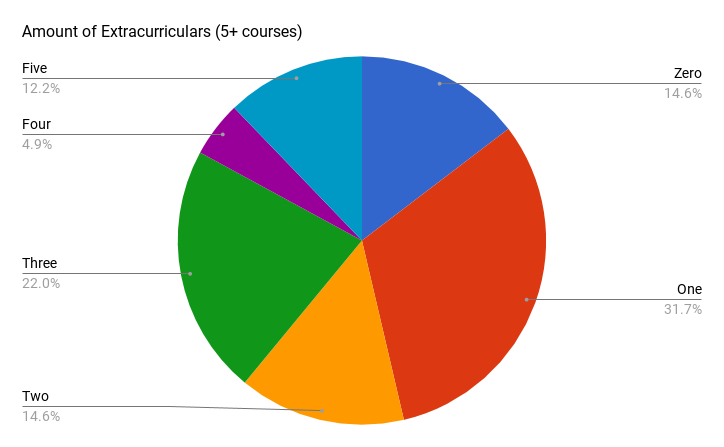
\includegraphics[width=1.0\textwidth]{sr-extracurric-pie-midgrad}
\caption{Results for extracurricular participation by amount of participation (mid to graduating students only).}
\end{figure}
\item \textit{Which of the following extracurricular activities, if any, pertain to you? }
Goal: Compare this answer to the same question on the post-deployment assessment. Ideally, RadGrad will increase the amount of student involvement in outside ICS-related activities due to providing students with stronger connections to the ICS community.
\begin{figure}[h]
\centering
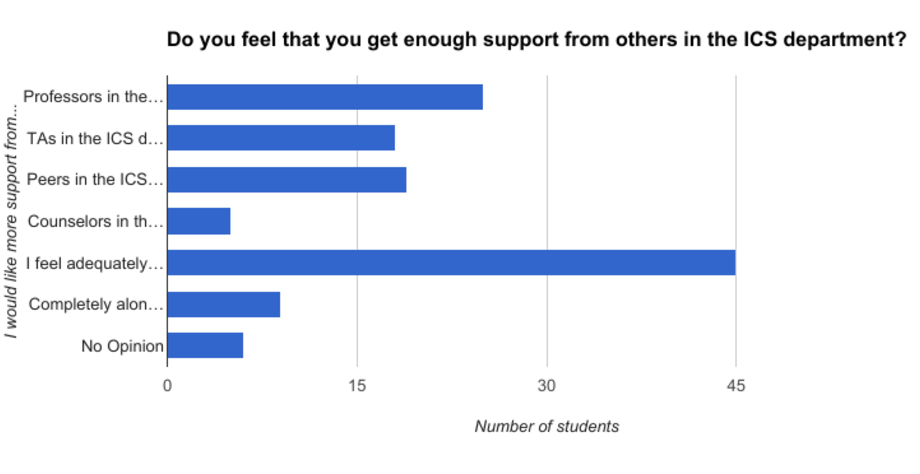
\includegraphics[width=1.0\textwidth]{sr-support-bar}
\caption{Results for support by types of support.}
\end{figure}

\begin{figure}[h]
\centering
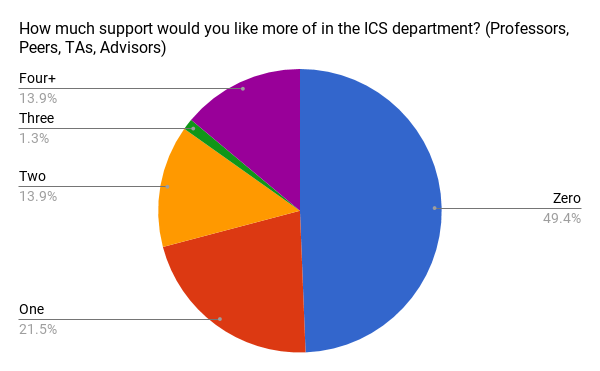
\includegraphics[width=1.0\textwidth]{sr-support-pie}
\caption{Results for support by amount of support desired}
\end{figure}
\item \textit{Do you feel that you get enough support from others in the ICS department?}
Goal: Are students lacking support in certain areas? How can RadGrad help to address this? Compare this answer to the same question on the post-deployment assessment. Ideally, RadGrad will provide a way to give more students the support they desire from others in the department. 
\begin{figure}[h]
\centering
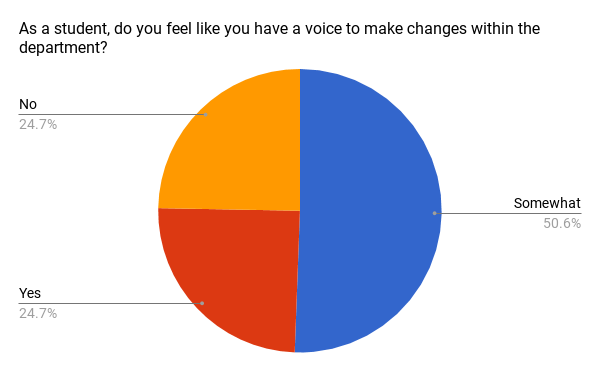
\includegraphics[width=1.0\textwidth]{sr-changes}
\caption{Results for feelings about having a voice to make changes.}
\end{figure}
\item \textit{As a student, do you feel like you have a voice to make changes within the department?}
Goal: If most students indicate that they do not feel like they have a voice within the department, what can RadGrad do to address this problem? Compare this answer to the same question on the post-deployment assessment. Ideally, RadGrad will cause more students to feel like they do have a voice to make changes in the department.
\begin{figure}[h]
\centering
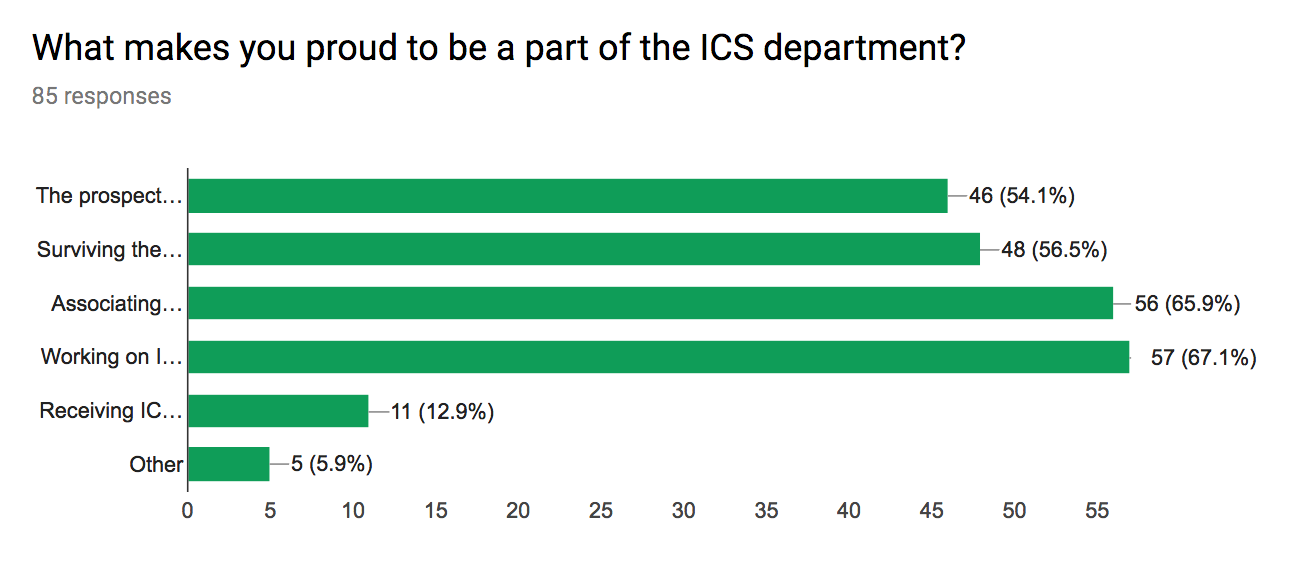
\includegraphics[width=1.0\textwidth]{sr-proud}
\caption{Results for reasons for being proud to be a part of the ICS department.}
\end{figure}
\item \textit{What makes you proud to be a part of the ICS department?}
Goal: This provides information about how current students view the department. A successful department should have a positive reputation among students, which can be manifested with a sense of pride. Compare this answer to the same question on the post-deployment assessment. Ideally, RadGrad will cause positive changes in the ICS department's reputation, leading to a greater sense of pride among students, which may play a role in students' success
\end{enumerate}

\section{Current ICS Students: Influences}
\begin{enumerate}
\begin{figure}[h]
\centering
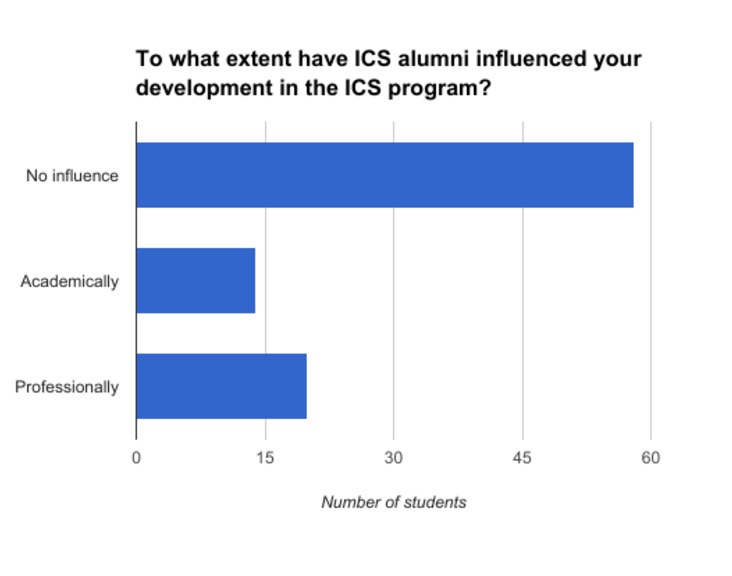
\includegraphics[width=1.0\textwidth]{sr-alumni-influence}
\caption{Results for alumni influence}
\end{figure}
\item \textit{To what extent have ICS alumni influenced your development in the ICS program?}
Goal: Compare this answer to the same question on the post-deployment assessment. Ideally, RadGrad will facilitate more student-alumni interaction, and cause more students to be influenced in some way by an alumn in an ICS-related way.
\begin{figure}[h]
\centering
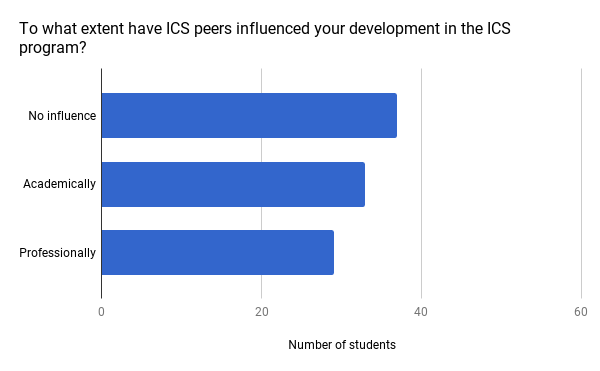
\includegraphics[width=1.0\textwidth]{sr-peer-influence}
\caption{Results for peer influence}
\end{figure}
\item \textit{To what extent have ICS peers influenced your development in the ICS program?}
Goal: Compare this answer to the same question on the post-deployment assessment. Ideally, RadGrad will facilitate more peer interaction, and cause more students to be influenced in some way by a peer in an ICS-related way.
\begin{figure}[h]
\centering
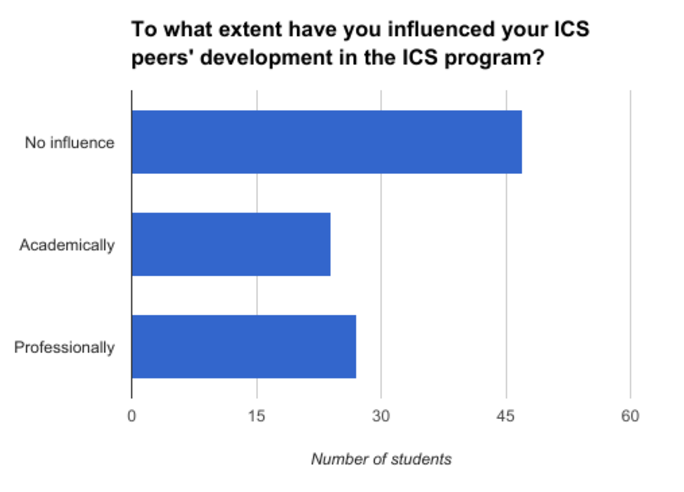
\includegraphics[width=1.0\textwidth]{sr-self-influence}
\caption{Results for student perceptions of their own influence}
\end{figure}
\item \textit{To what extent have you influenced your ICS peers’ development in the ICS program?}
Goal: Compare this answer to the same question on the post-deployment assessment. Ideally, RadGrad will facilitate more peer interaction, and cause more students play a role in influencing their peers in an ICS-related way.
\end{enumerate}

\section{Graduating ICS Students}
\begin{enumerate}
\begin{figure}[h]
\centering
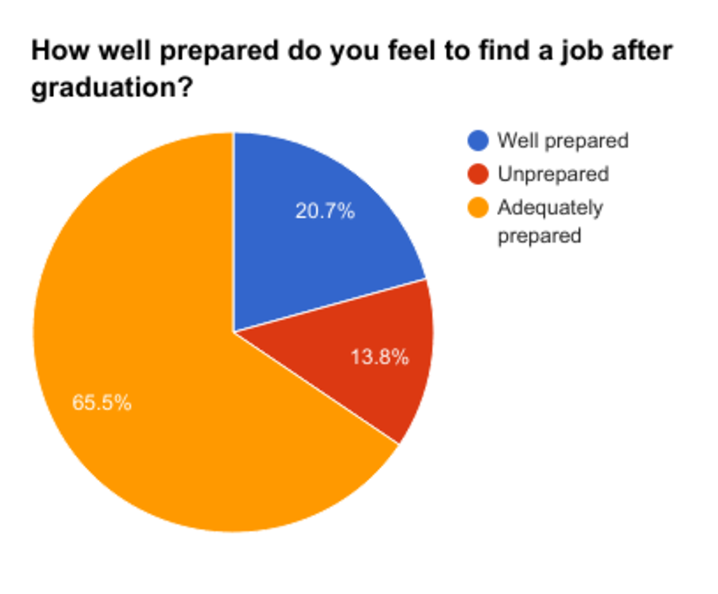
\includegraphics[width=1.0\textwidth]{sr-prepared}
\caption{Results for graduation preparedness.}
\end{figure}
\item \textit{Now that you are nearing the end of your ICS degree program experience, how well prepared do you feel to find a job after graduation?}
Goal: If the ICS department is fulfilling its duty, most graduating students should feel at least adequately prepared (ideally well prepared) for the future. If most students indicate that they do not feel prepared, what can RadGrad do to address this problem? Ideally, after deploying RadGrad, a higher percentage of students will feel either adequately prepared or well prepared for the future.
\begin{figure}[h]
\centering
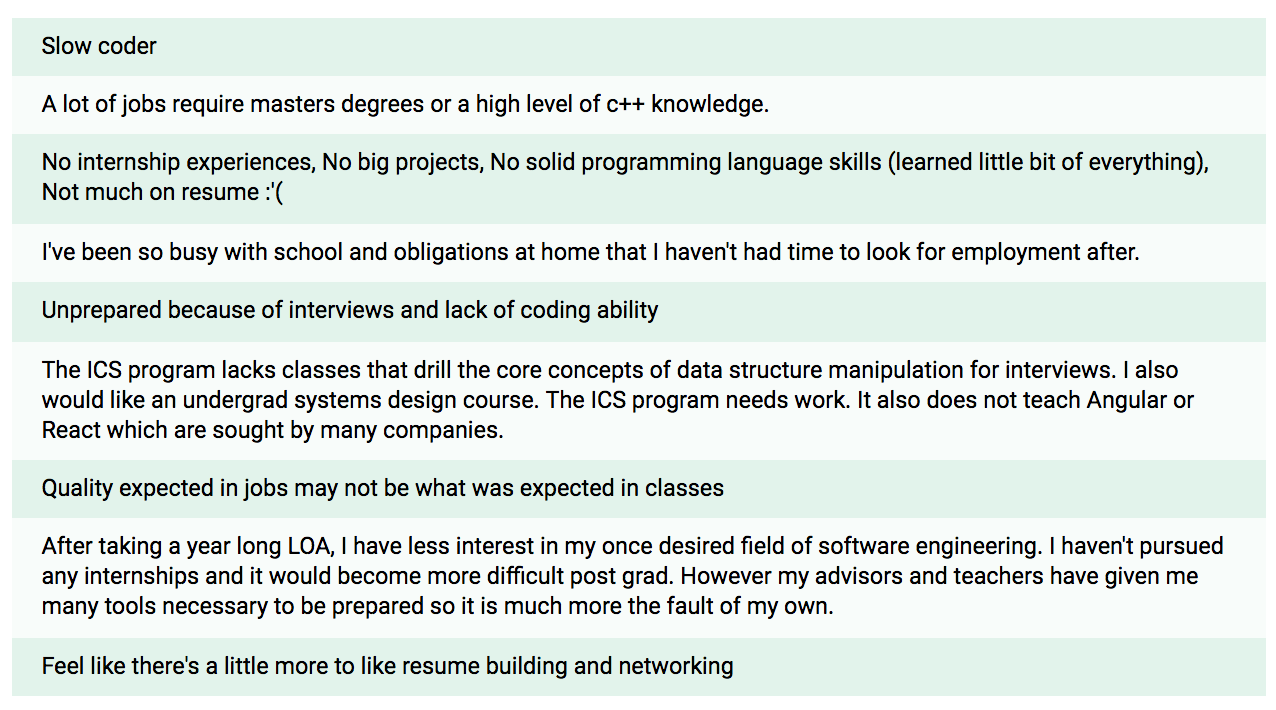
\includegraphics[width=1.0\textwidth]{sr-unprepared-grad-reasons}
\caption{Reasons for not feeling prepared for graduation.}
\end{figure}
\item \textit{If you answered above that you feel unprepared to find a job after graduation, please explain why. }
Goal: Are there any common reasons for students not feeling prepared? If so, is there anything RadGrad can do to address this problem? Ideally, after deploying RadGrad, there will be a lower percentage of students who indicate the same problems as the preliminary questionnaire. 
\end{enumerate}


